\item Dois carros $A$ e $B$ têm massa de \SI{2000}{\kilogram} e colidem no pavimento escorregadio de um cruzamento. A direção do movimento de cada carro após a colisão é medida pelos rastros deixados, como mostrado. Se o motorista $A$ afirma que vinha a \SI{15}{\meter/\second} (\SI{54}{\kilo\meter/\hour}) imediatamente antes da colisão e que, após a mesma, acionou os freios de modo que o carro derrapou \SI{3}{\meter} antes de parar, determine a velocidade aproximada do carro $B$ imediatamente antes da colisão. Suponha que o coeficiente de atrito cinético entre as rodas do carro e o pavimento é $\mu_{k}=0.15$. \textit{Nota:} a linha de impacto não é definida; no entanto, essa afirmação não é necessária para a solução.

\begin{flushright}
	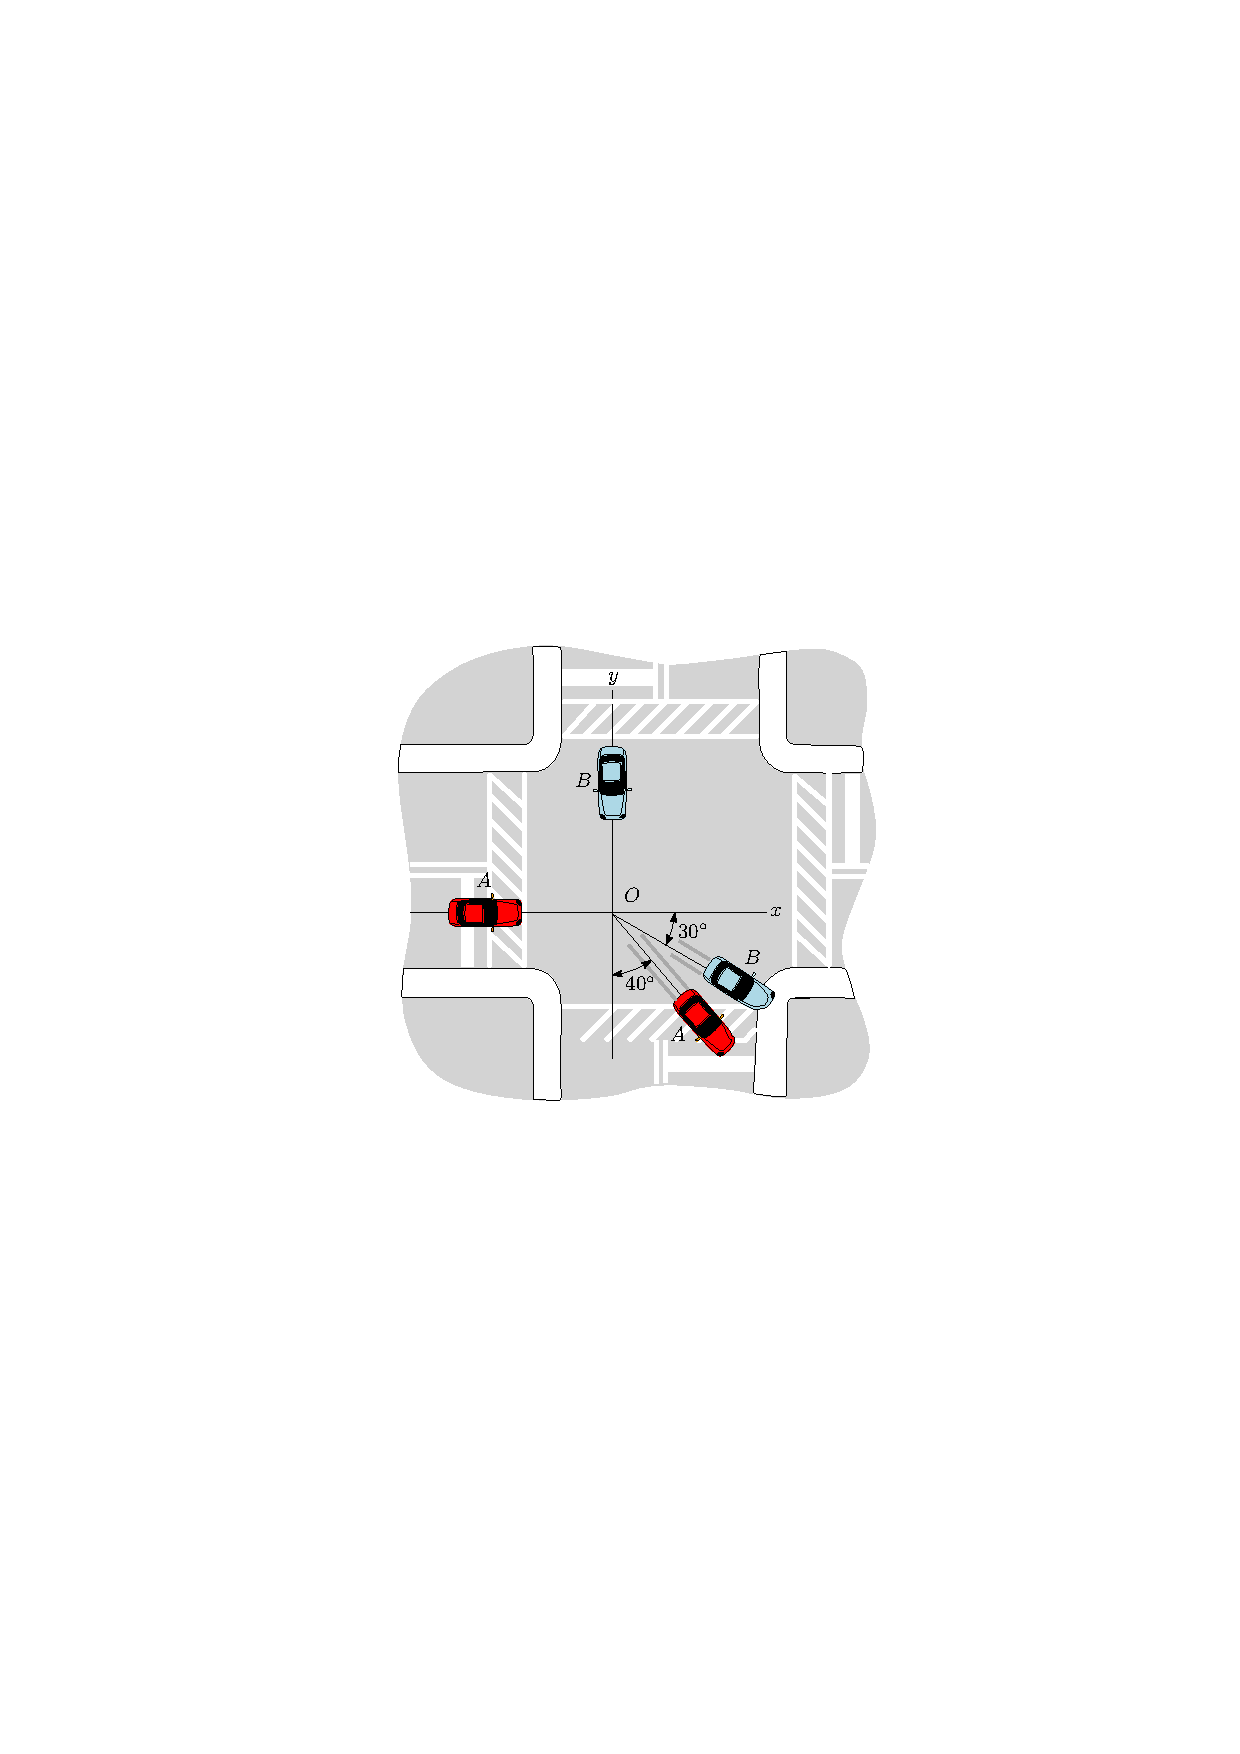
\includegraphics[scale=1.2]{images/draw_14}
\end{flushright}